\paragraph{Number of segregating sites.} Another measure of genetic variability is the total number of sites
that are polymorphic (segregating) in our sample. One issue is that
the number of segregating sites will grow as we sequence more
individuals (unlike $\pi$). Later in the course, we'll talk about how to standardize the
number of segregating sites for the number of individuals sequenced (see \eqn \eqref{watterson_theta}).

\paragraph{The frequency spectrum.}
We also often want to compile information about the frequency of
alleles across sites.  We call alleles that are found once in a sample
\emph{singletons}, alleles that are found twice in a sample {\emph
  doubletons}, and so on. We count up the number of loci where an
allele is found $i$ times out of $n$, e.g. how many singletons are
there in the sample, and this is called the \emph{frequency
  spectrum}. We'll want to do this in some consistent manner, such as calculating the frequency spectrum of the minor allele or the derived allele.

\begin{question}{}
How many minor-allele singletons are there in \textit{D. simulans} in
the ADH region? [Defining minor allele just within \textit{D. simulans}.]
%JRI: ambiguous. is the minor allele defined across all species or just within simulans?
\erin{students were confused whether you are defining 'minor allele' with reference to the species or to the whole group. There are no major allele singletons with reference to the individual species, but I think it's confusing because the only example of a minor allele given in the text by its definition is the 'minor allele in D. melanogaster' .. maybe it would be best to clarify in the question or just give an example of the minor allele in the whole sample instead.}
 \end{question}
\paragraph{Levels of genetic variability across species.}
Two observations have puzzled population geneticists since the
inception of molecular population genetics. The first is the relatively high
level of genetic variation observed in most obligately sexual species.
This first observation, in part, drove the development of the Neutral
theory of molecular evolution, the idea that much of this molecular
polymorphism may simply reflect a balance between genetic drift and
mutation.
The second observation is the relatively narrow range of
polymorphism across species with vastly different census sizes. This
observation represented a puzzle as the Neutral theory predicts that
levels of genetic diversity should scale with population size. Much effort
in theoretical and empirical population genetics has been devoted to
trying to reconcile models with these various observations. We'll
return to discuss these ideas throughout our course.
%Neutral

\begin{marginfigure}[-1cm]
\begin{center}
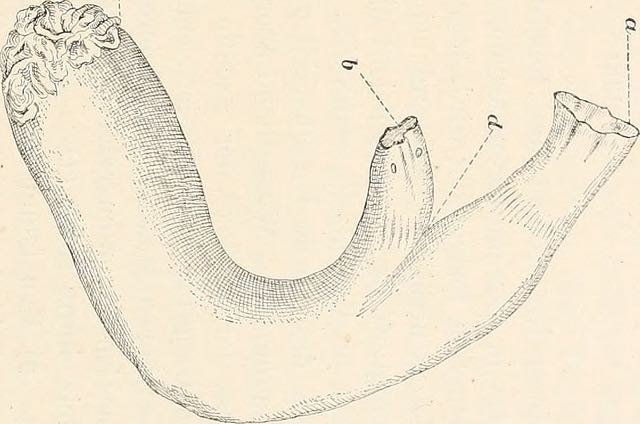
\includegraphics[width= 0.8 \textwidth]{illustration_images/alleles_genotypes/Ciona_intestinalis/21016139168_2a8a57ded3_z.jpg}
\end{center}
\caption{Sea Squirt ({\it Ciona intestinalis}). \BHLNKC{Einleitung in die vergleichende gehirnphysiologie und
  Vergleichende psychologie. Loeb, J. 1899.}{https://www.flickr.com/photos/internetarchivebookimages/21016139168/in/photolist-y28cZ3-xatkQu-w6Ki9C-wLcTJy-tLanR7-wKRZbh-w79C6u-toKNq1-u3ojn3-y8KsPP-xK7CZj-bu2usR-wLkfdM-wbkfau-x8n51o-ygpRAN-xMgGnk-towSTe-xQtix3-xMrift-wQoMNq-y51RxU-xPH4Cu-x4uB1v-xPGVFs-x4GN5a-y6rT8N-y6Aous-y7jV9n-yb6s66-x7F6Wh-y7upRp-xkz9VY-u1qerd-wYE4Cz-y5aH2Y-y7uJpM-xPSvFU-y6ALo7-xPZ3FM-xPHUef-yaa3dw-xPSKSC-w7A1aj-x4bgsH-tLas4q-x1e1dv-w7BkZB-xrQxFJ-y8acDr}{MBLWHOI Library}} \label{fig:ciona}
\end{marginfigure}

The first observations of molecular genetic diversity within natural populations were made from surveys of allozyme data, but we can revisit these general patterns with modern data. For
example, \citet{leffler:12} compiled data on levels of within-population,
autosomal nucleotide diversity ($\pi$) for 167 species across 14 phyla from
non-coding and synonymous sites (Figure \ref{fig:Leffer}). The species with the lowest levels of
$\pi$ in their survey was Lynx, with $\pi = 0.01\%$, i.e. only
$1/10000$ bases differed between two sequences. In contrast, some of the highest levels of
diversity were found in {\textit{Ciona savignyi}, Sea Squirts, where a remarkable
$1/12$ bases differ between pairs of sequences. This $800$-fold range of
diversity seems impressive, but census population sizes have a much
larger range.
%JRI: I feel like an example of census size would be useful. the genus Cyclothone, which exists in the trillions, comes to mind as a surprising example that you could compare to like a coelocanth: https://commons.wikimedia.org/wiki/File:Wissenschaftliche_Ergebnisse_der_Deutschen_Tiefsee-Expedition_auf_dem_Dampfer_%22Valdivia%22_1898-1899_(Tafel_6)_(7413855904).jpg
\begin{figure*}
\begin{center}
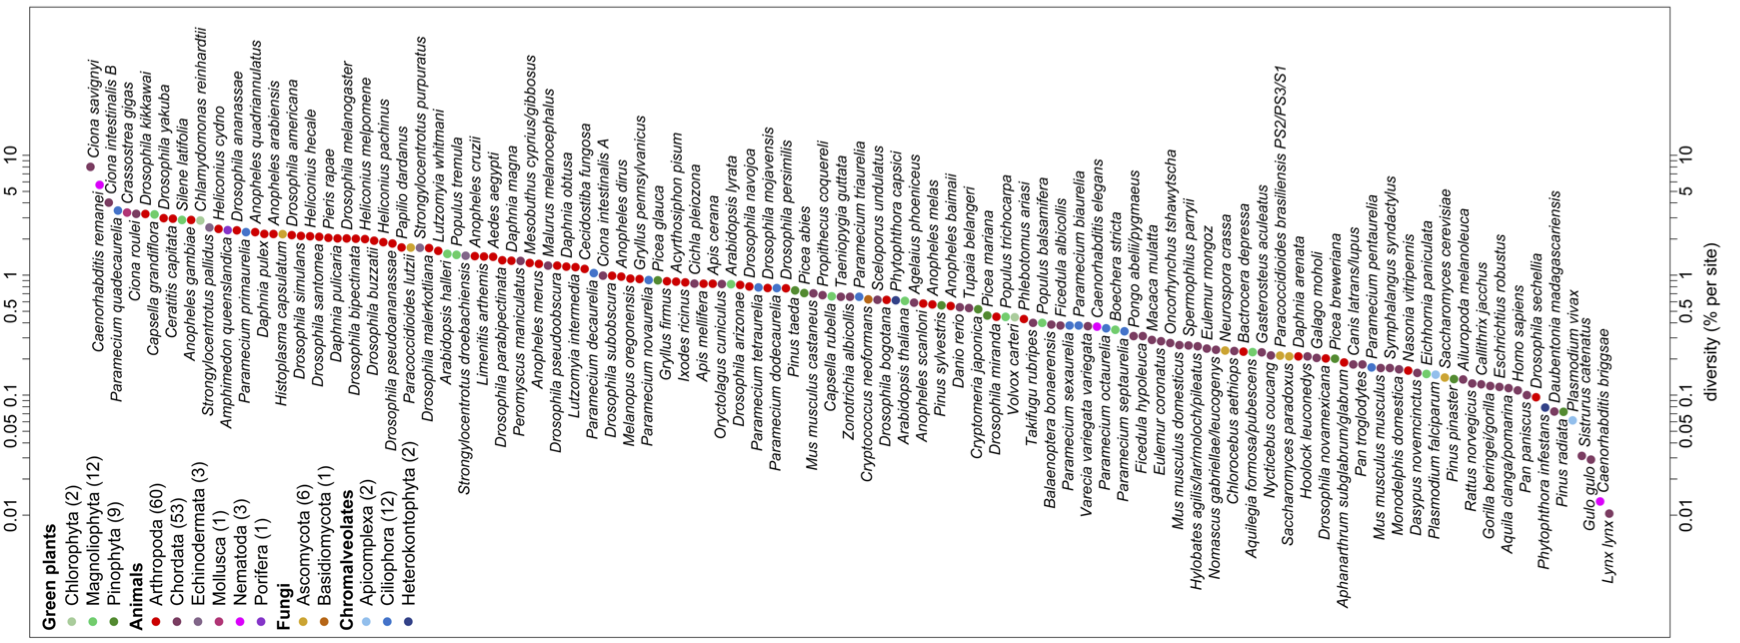
\includegraphics[width= \textwidth]{Journal_figs/alleles_genotypes/Leffer_riddle/Leffer_riddle_diversity.png}
\end{center}
\caption{Levels of autosomal nucleotide diversity for 167
species across 14 phyla. Figure 1 from \citet{leffler:12}, \PLOSccBY. Points are
ranked by their $\pi$, and coloured by their phylum. Note the log-scale.} \label{fig:Leffer}
\end{figure*}

\begin{marginfigure}[2cm]
\begin{center}
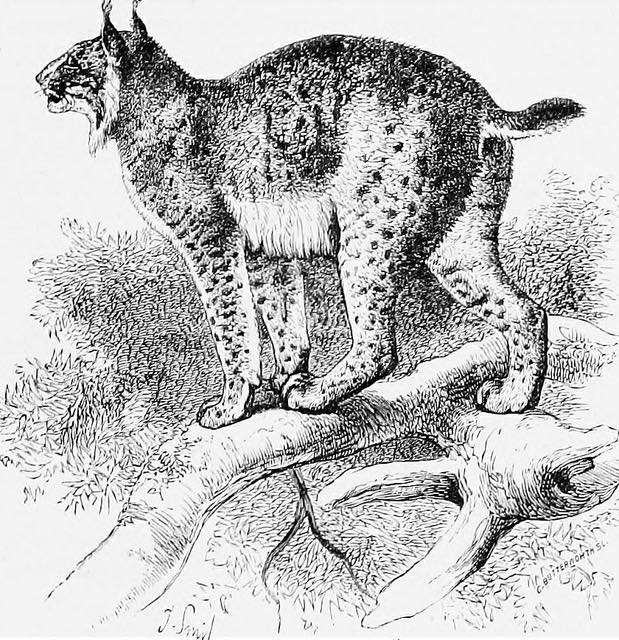
\includegraphics[width= 0.8 \textwidth]{illustration_images/alleles_genotypes/Lynx/20731949565_8a065700af_z.jpg}
\end{center}
\caption{Eurasian Lynx (\textit{Lynx lynx}). \BHLNKC{An introduction to the study
  of mammals living and extinct. Flower, W.H. and Lydekker, R. 1891.}{https://www.flickr.com/photos/internetarchivebookimages/20731949565/in/photolist-x5Jzv2-x6QVyp-xir9rH-wYHrQD-wPn1sP-w9PsqY-xDcqri-sMcQoB-trrkVd-x6Nx1H-wPea7N-sM28N9-tJ3zsp-xneVdx-wGJRtQ-xnfHZ8-wPfga7-xCUPrN-x7kXDV-xmAb9E-xm3x4k-xBoSKb-wGTgyB-xBoSbf-wGGvzA-xmzYTJ-oeKJcH-xA1Ffr-xA1Eji-xqWTQZ-xF4Lru-oxJfrH-x7ojSn-xra8zP-wGGibY-xgb21y-xY1jH9-xY1iyf-wGHxTS-wGQEoR-xmtPQh-x8uFKK-xdTkoU-wPggQf-wPfvHN-wPfc27-w9YnGF-wPeauS-wPiVxK-w6aiSi}{Cornell University Library}} \label{fig:Lynx}
\end{marginfigure}

\subsection{Hardy--Weinberg proportions}
Imagine a population mating at random with respect to genotypes, i.e. no
inbreeding, no assortative mating, no population structure, and no sex differences
in allele frequencies. The frequency of allele $A_1$ in the population at the
time of reproduction is $p$. An $A_1A_1$ genotype is made by reaching out into
our population and independently drawing two $A_1$ allele gametes to form a
zygote. Therefore, the probability that an individual is an $A_1A_1$ homozygote
is $p^2$. This probability is also the expected frequencies of the $A_1A_1$
homozygote in the population. The expected frequency of the three possible
genotypes are

\marginnote{Throughout this chapter we'll be making use of the basic
  rules of probability to find the probabilities of combinations of
  events, e.g. the alleles found in an individual, see Appendix \ref{Section_rules_prob} for a refresher.}

%\begin{table}[htp!]
\begin{center}
\begin{tabular}{ccc}
\hline
$f_{11}$ & $f_{12}$ & $f_{22}$ \\
\hline
$p^2$ & $2pq$ & $q^2$ \\
\end{tabular}
\end{center}
%\caption{\textbf{Hardy Weinberg}} \label{table:HWE}
% \end{table}
i.e. their Hardy-Weinberg expectations \citep{hardy1908mendelian,weinberg1908ber}.
Note that we only need to assume random mating with respect to our
focal allele in order for these expected frequencies to hold in the
zygotes forming the next generation. Evolutionary forces, such as
selection, change allele frequencies within generations, but do not
change this expectation for new zygotes, as long as $p$ is the
frequency of the $A_1$ allele in the population at the time when
gametes fuse. We only need the assumptions of no migration, selection,
and mutation in order for these Hardy-Weinberg expectations of
genotypes to represent a long term equilibrium.


\begin{question}{}
On the coastal islands of British Columbia there is a subspecies of
black bear (\textit{Ursus americanus kermodei}, Kermode's bear). Many members of this
black bear subspecies are white; they're sometimes called spirit bears. These
bears aren't hybrids with polar bears, nor are they albinos. They are
homozygotes for a recessive change at the MC1R gene. Individuals who
are $GG$ at this SNP are white, while $AA$ and $AG$ individuals are black.

Below are the genotype counts for the MC1R polymorphism in a
sample of bears from British Columbia's island populations from \citet{RITLAND:01}.
\begin{center}
\begin{tabular}{ccc}
\hline
$AA$ & $AG$ & $GG$ \\
\hline
42 & 24 & 21\\
\end{tabular}
\end{center}
What are the expected frequencies of the three genotypes under HW?
\end{question}

\begin{marginfigure}    %%%New Kermode_bear
                        %%%https://twitter.com/BioDivLibrary/status/1191354772034592774/photo/3
                        %%%page 77 https://www.biodiversitylibrary.org/item/38166?utm_source=Twitter&utm_medium=social+media&utm_term=&utm_content=MBLWHOI&utm_campaign=Mammal+Monday#page/114/mode/1up
  \begin{center}
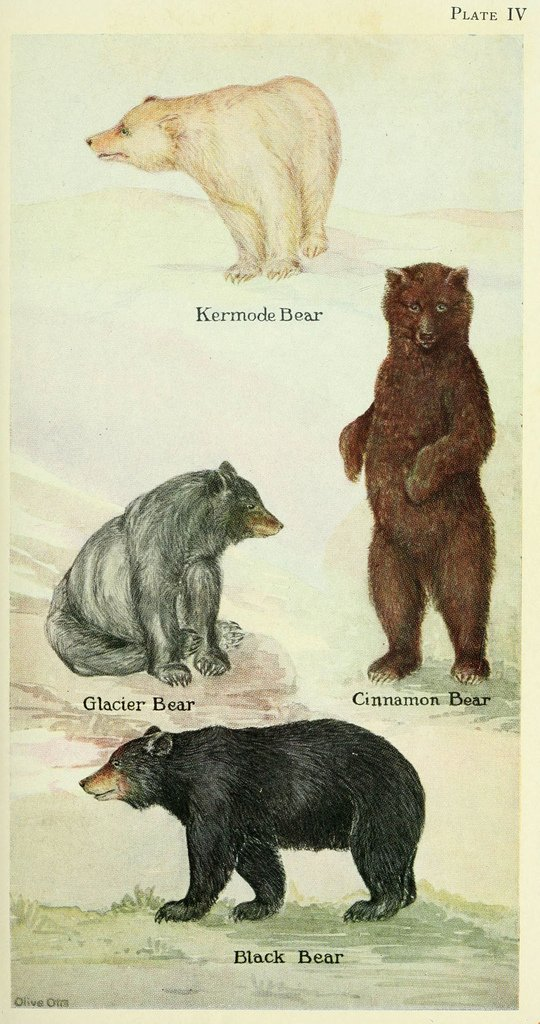
\includegraphics[width= \textwidth]{illustration_images/alleles_genotypes/Kermode_bear/EIiK2dsWoAAmUOf.jpeg}  
%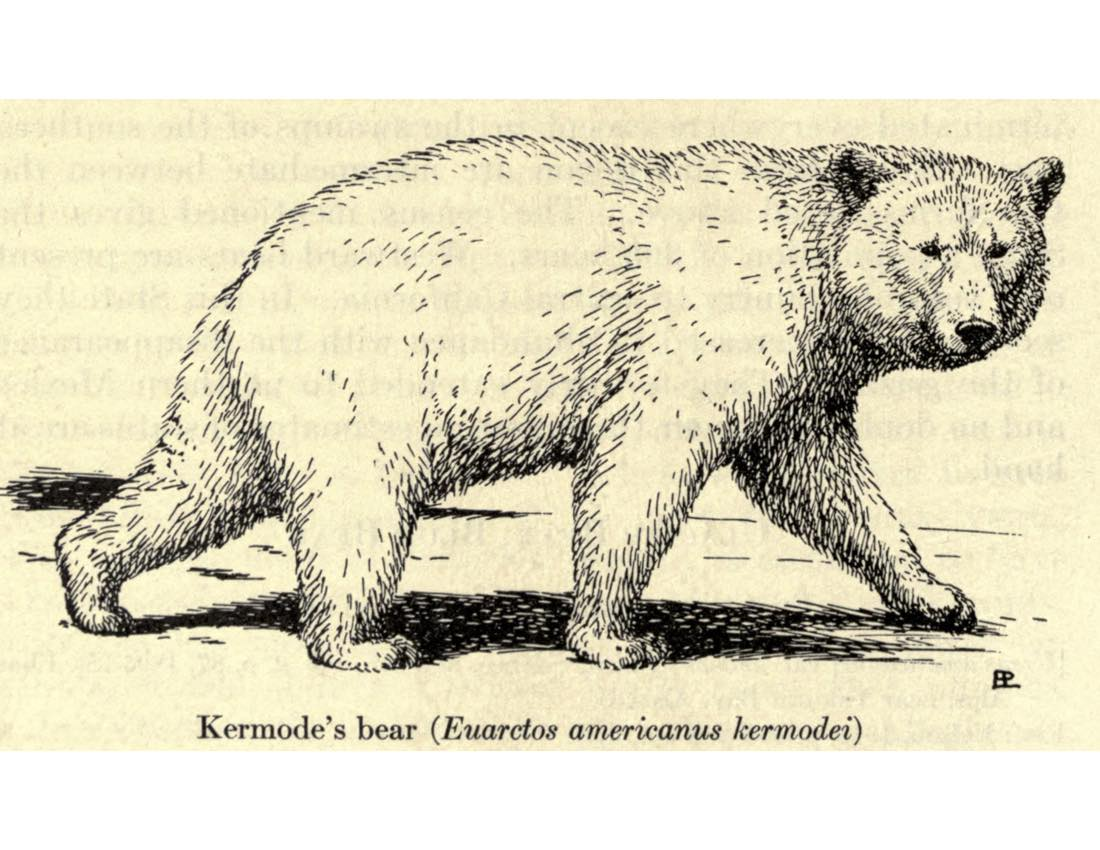
\includegraphics[width= \textwidth]{illustration_images/alleles_genotypes/Kermode_bear/Kermode_bear.jpg}
\end{center}
\caption{Kermode's bear (\textit{Ursus americanus kermodei}). It's
  possible that this morph is favoured as the salmon these bears eat have a harder time
  seeing the light morph \citep{klinka2009adaptive}. The adaptive
  value of tasting like cinnamon is unknown. \BHLNKC{Field book of North American mammals;
    descriptions of every mammal known north of the Rio
    Grande. Anthony, (1928) H. E.}{https://www.biodiversitylibrary.org/item/38166\#page/115/mode/1up}{MBLWHOI Library} } \label{fig:Kermodes_bear}
%\caption{Kermode's bear. \BHLNC{Extinct and vanishing mammals of the western
 % hemisphere. 1942. Glover A.}{https://www.biodiversitylibrary.org/page/20699033\#page/160/mode/1up}{Prelinger
%  Library} } \label{fig:Kermodes_bear}
\end{marginfigure}

%JRI: I think you mean under HW not HWE.  i think somewhere you should introduce HW in a parenthetical"Hard--Weinberg  (HW) proportions" etc. just to be abdunantly clear what the acronym means. also the ritland citation isn't showing year for some reason.


See Figure \ref{fig:HWE_CEU_YRI} for a nice
empirical demonstration of Hardy--Weinberg proportions. The mean
frequency of each genotype
closely matches its HW expectations, and much of the scatter of the
dots around the expected line is due to our small sample size ($\sim
60$ individuals). While HW often
seems like a silly model, it often holds remarkably well within
populations. This is because individuals don't mate at random, but they
do mate at random with respect to their genotype at most of the loci
in the genome.

\begin{question}{}
You are investigating a locus with three alleles, A, B, and C, with
allele frequencies $p_A$, $p_B$, and $p_C$. What fraction of the
population is expected to be homozygotes under Hardy--Weinberg?
\end{question}

Microsatellites are regions of the genome where individuals vary for
the number of copies of some short DNA repeat that they carry. These
regions are often highly variable across individuals, making them
a suitable way to identify individuals from a DNA sample. This
so-called DNA fingerprinting has a range of applications from
establishing paternity and identifying human remains to matching
individuals to DNA samples from a crime scene. The FBI make use of the
CODIS database\sidenote{CODIS: Combined DNA Index System}. The CODIS
database contains the genotypes of over 13 million people, most of
whom have been convicted of a crime. Most of
the profiles record genotypes at 13 microsatellite loci that are
tetranucleotide repeats (since 2017, 20 sites have been genotyped).

The allele counts for two loci (D16S539
and TH01) are shown in table \ref{table:CODIS_1} and
\ref{table:CODIS_2} for a sample of 155 people of European ancestry. You can assume these two loci are on different chromosomes.